\documentclass{standalone}

\usepackage{tikz}

\begin{document}
	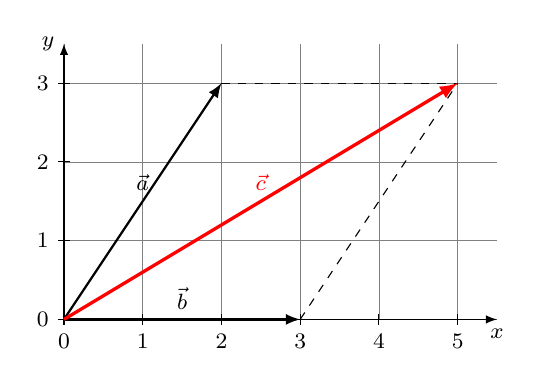
\begin{tikzpicture}
		[
		x=1cm, y=1cm, scale=1.0, font=\footnotesize, >=latex 
		%Voreinstellung für Pfeilspitzen
		]
		
		%Raster im Hintergrund
		\draw[step=1, gray, very thin] (0,0) grid (5.5,3.5);
		
		%Zahlen auf x-Achse
		\foreach \x in {0,1,2,3,4,5}
		\draw[shift={(\x,0)},color=black] (0pt,2pt) -- (0pt,-2pt) node[below]
		{\footnotesize $\x$};
		
		%Länge x Achse
		\draw [-latex] (0,0) -- ++(5.5,0) node[below] {$x$};
		
		%Länge y Achse
		\draw [-latex] (0,0) -- ++(0,3.5) node[left] {$y$};
		
		%Zahlen auf y-Achse 
		%\foreach \y in {0,...,1}
		\foreach \y in {0,1,2,3}
		\draw[shift={(0,\y)},color=black] (2pt,0pt) -- (-2pt,0pt) node[left]
		{\footnotesize $\y$};		
		
		%Vektor a
		\draw[-latex, thick] (0,0) -- (2,3) node [midway, above] {$\vec{a}$} node (a) {}; 
		%Vektor b
		\draw[-latex, thick] (0,0) -- (3,0) node [midway, above] {$\vec{b}$} node (b) {}; 
		\draw[dashed] (a.center) -- ++ (3,0) node (c) {};
		\draw[dashed] (b.center) -- ++ (2,3);
		\draw[very thick, red, -latex] (0,0) -- (c.center) node [midway, above] {$\vec{c}$};
	\end{tikzpicture}
\end{document}